\documentclass{article}

\usepackage{url}
\usepackage{nicefrac}
\usepackage{amssymb,amsfonts,amsmath,amsthm}
\usepackage{mathtools}
\usepackage{adjustbox}
\usepackage{bm}
\usepackage{bbold}
\usepackage[margin=60pt]{geometry}
\pdfinclusioncopyfonts=1

\usepackage{xcolor}
\definecolor{RED}{HTML}{EB6231}
\definecolor{YELLOW}{HTML}{E29D26}
\definecolor{BLUE}{HTML}{5D80B4}
\definecolor{LIGHTGREEN}{HTML}{6ABD9B}
\definecolor{GREEN}{HTML}{8FB03E}
\definecolor{PURPLE}{HTML}{BE1E2D}
\definecolor{BROWN}{HTML}{A97C50}
\definecolor{PINK}{HTML}{DA1C5C}

\newcommand{\specialcell}[2][c]{%
	\begin{tabular}[#1]{@{}c@{}}#2\end{tabular}}

\newcommand{\der}{\mathrm{d}}
\newcommand{\e}{\mathrm{e}}
\newcommand{\dnds}{dN/dS}
\newcommand{\indice}{l}
\newcommand{\indiceexp}{^{(\indice)}}
\newcommand{\angstrom}{\text{\normalfont\AA}}

% Time, effective population size and mutation rate.
\newcommand{\Ne}{N_{\mathrm{e}}}
\newcommand{\Nsite}{S}
\newcommand{\site}{\text{s}}
% DNA

\newcommand{\ci}{{i}}
\newcommand{\cj}{{j}}
\newcommand{\itoj}{\ci, \cj}
\newcommand{\nucitoj}{\ci \rightarrow \cj}
\newcommand{\submatrix}{Q}

\begin{document}

\part*{Simulations}

\section{Simulation with independent fitness profiles}
\begin{center}
	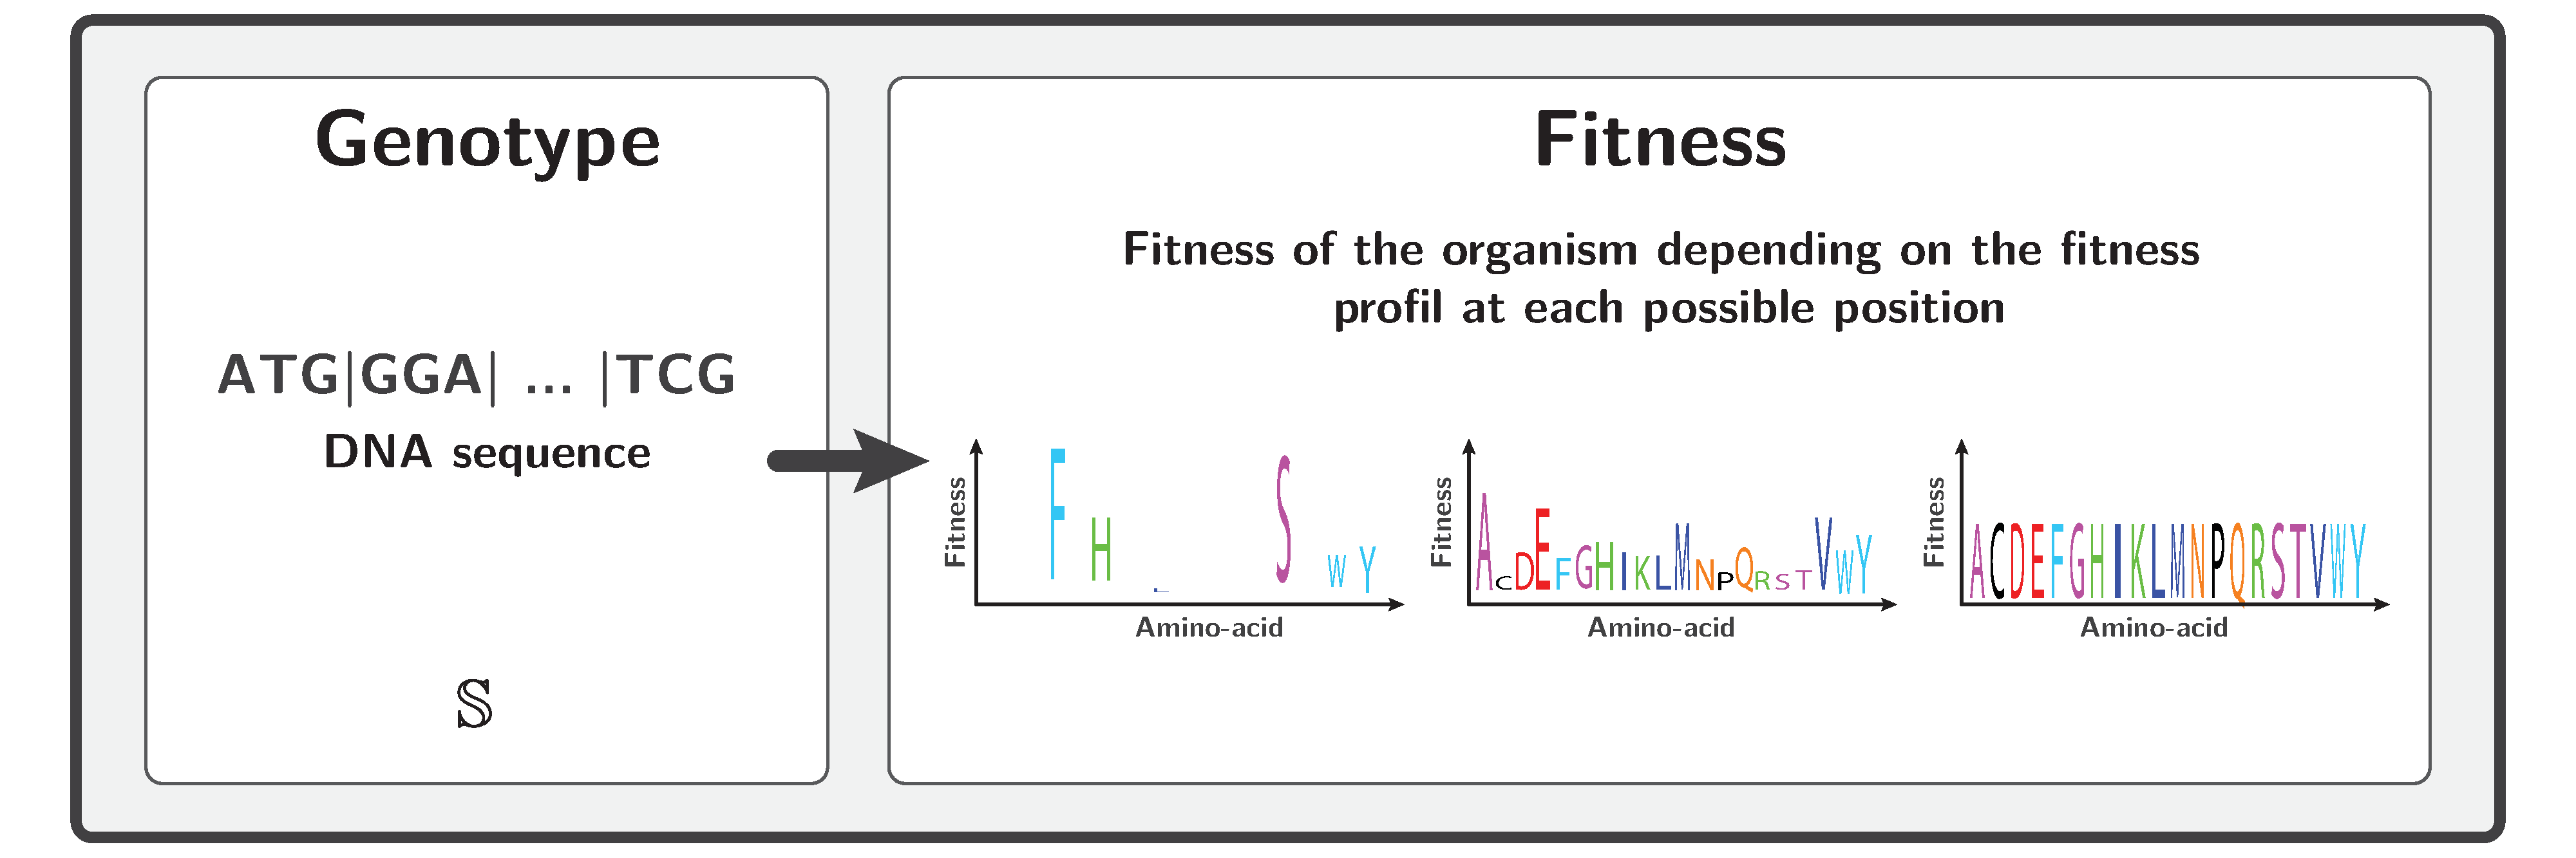
\includegraphics[width=165mm] {artworks/ModelSimuDiv.pdf}
\end{center}

\section{Simulation in Wright-Fisher context}
\begin{center}
	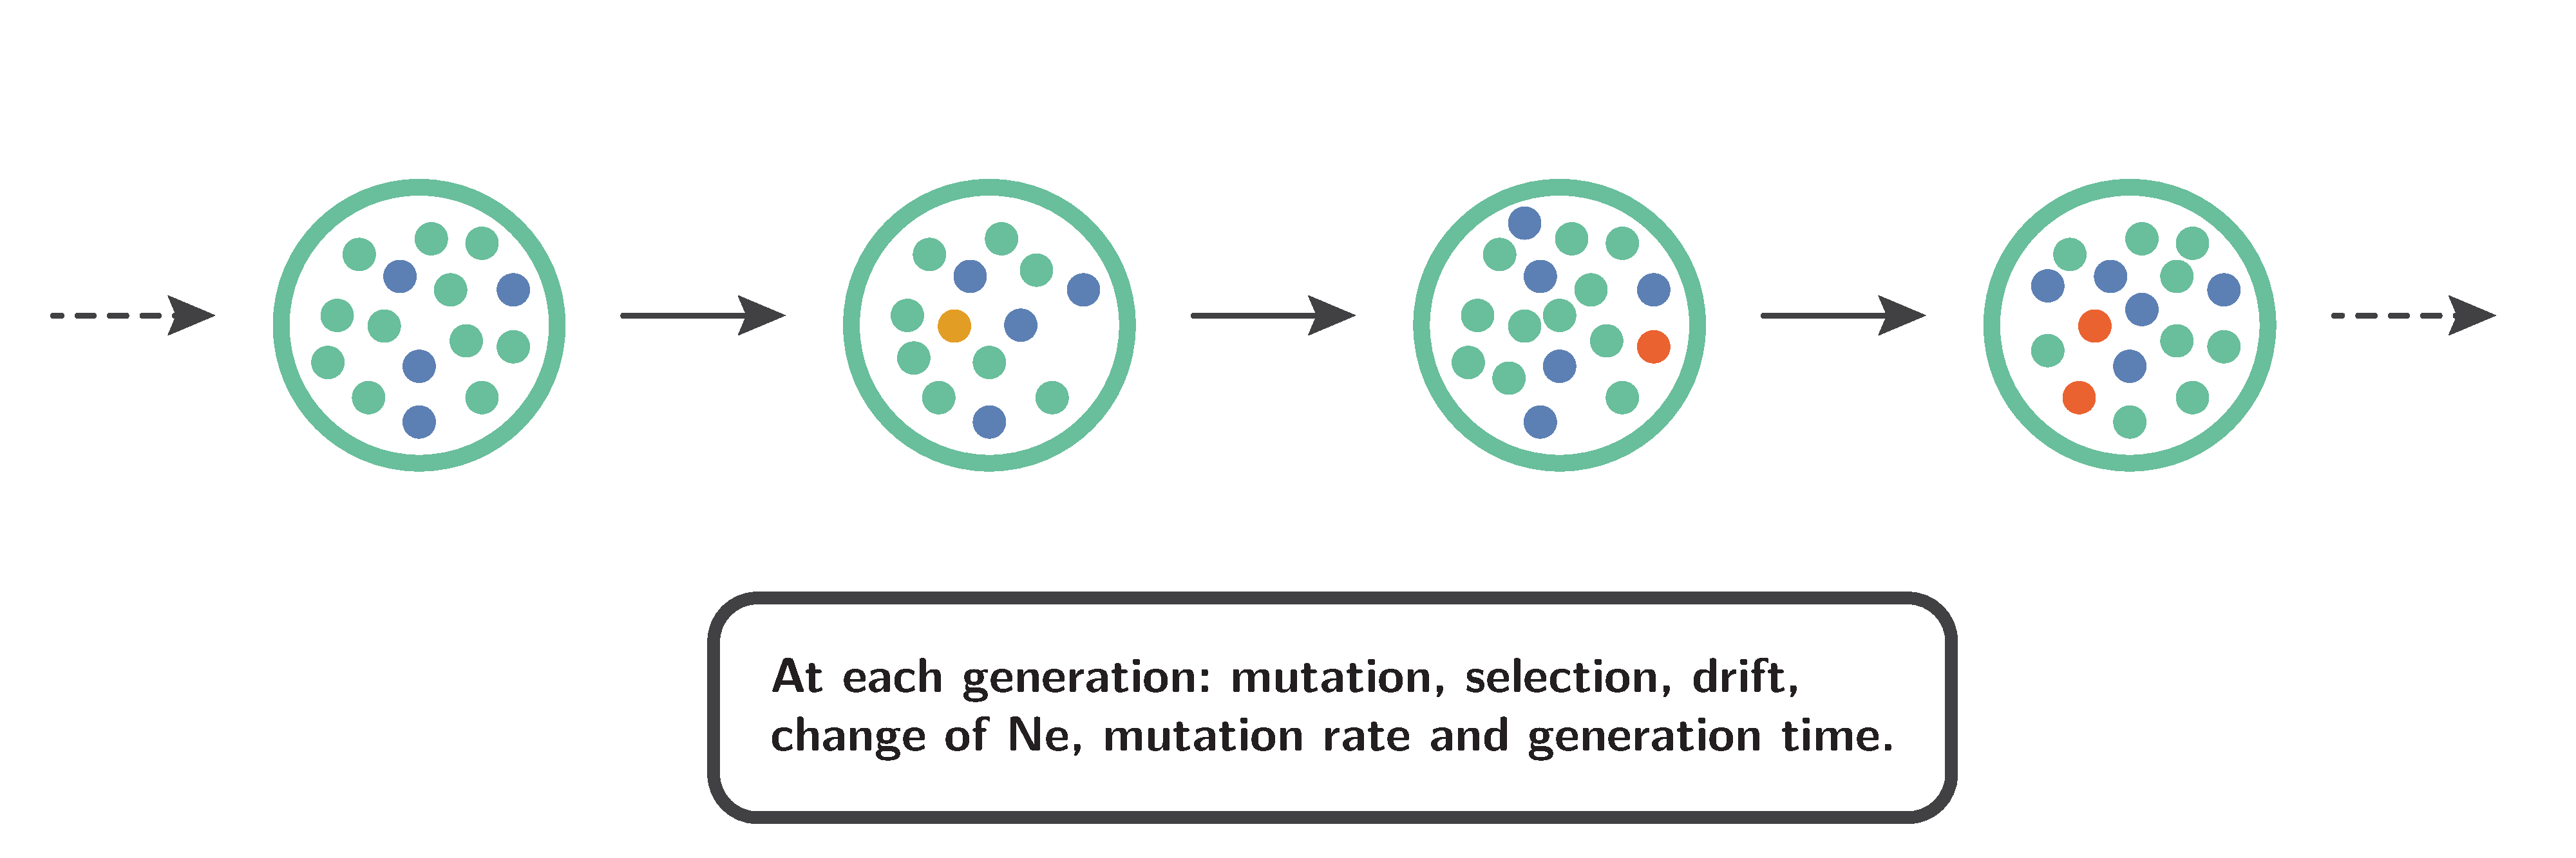
\includegraphics[width=165mm] {artworks/ModelSimuPoly.pdf}
\end{center}

\section{Simulation with Fisher geometric landscape}
\begin{center}
	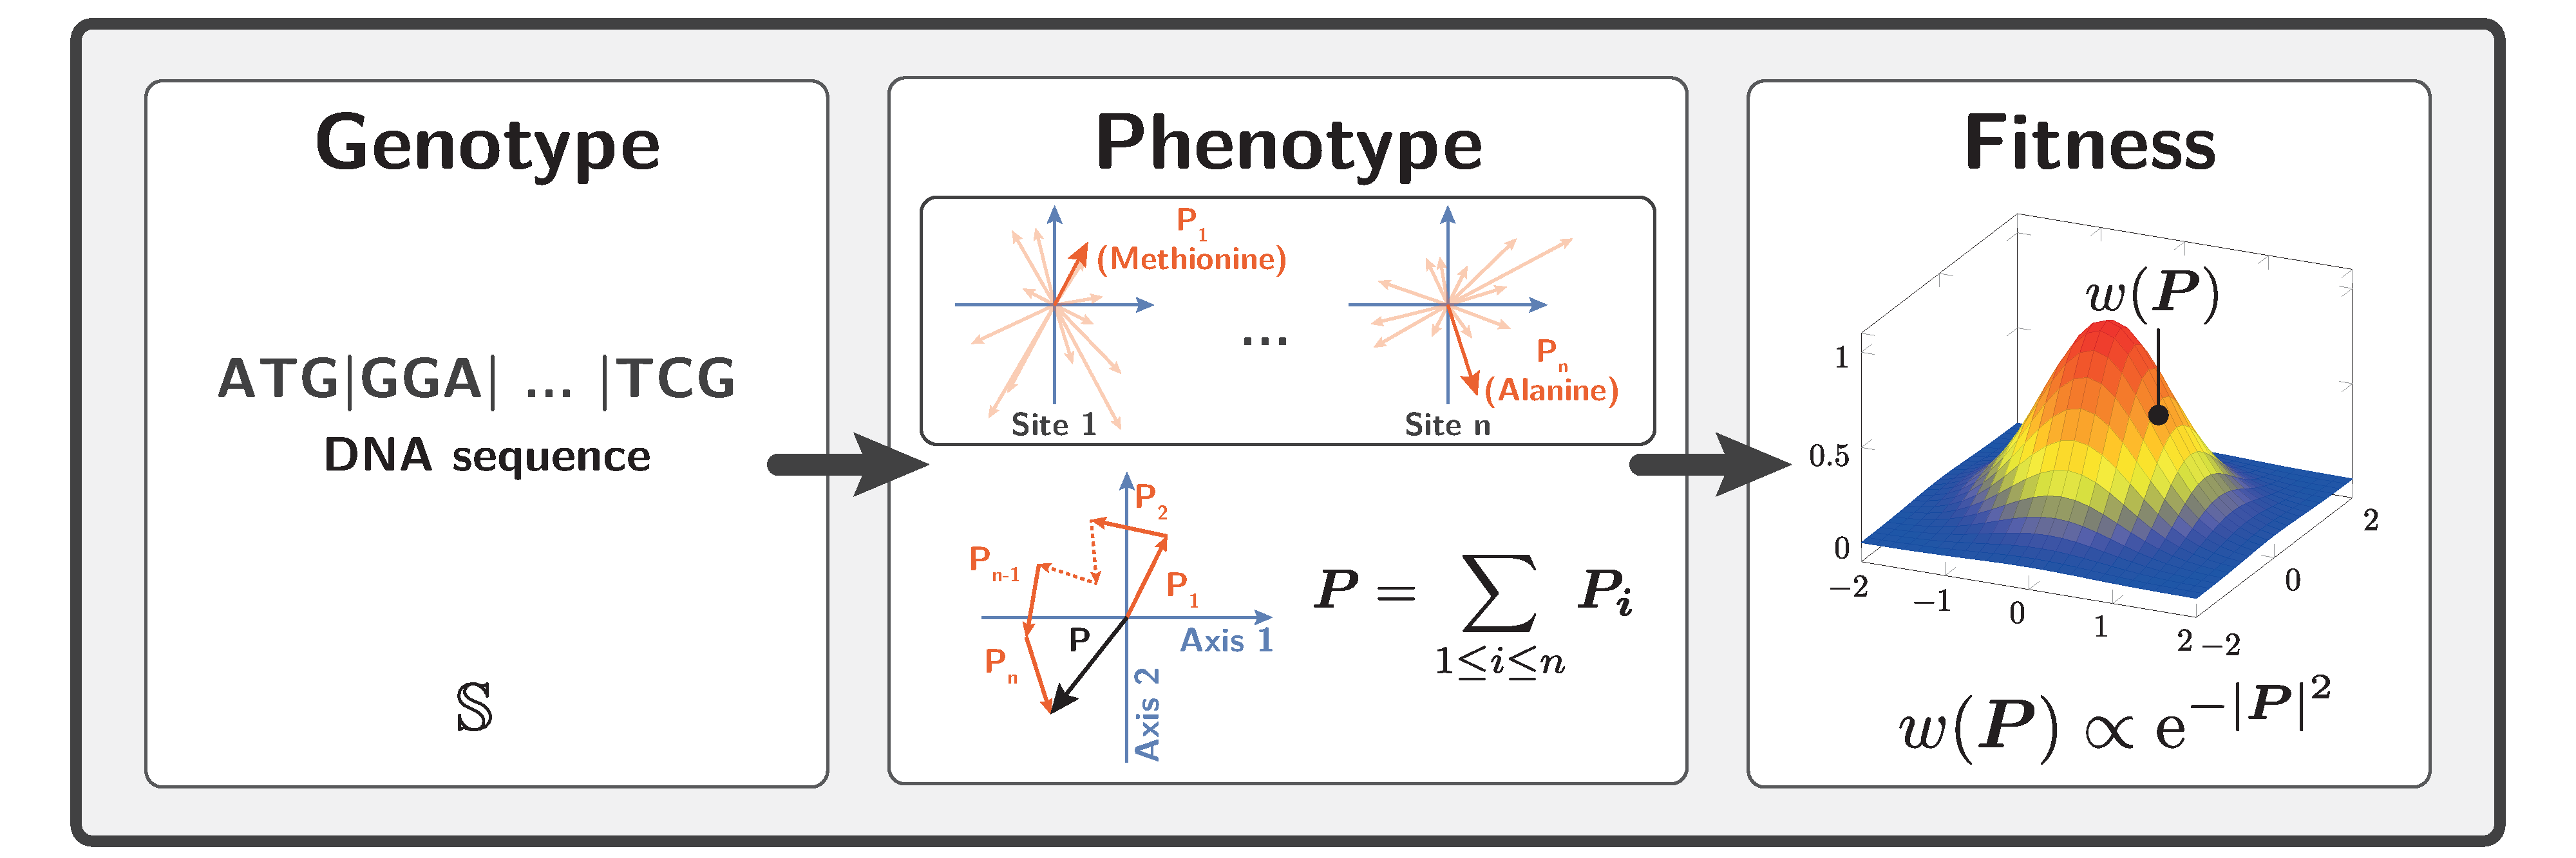
\includegraphics[width=165mm] {artworks/ModelSimuGeo.pdf}
\end{center}

\section{Simulation with protein folding probability}
We simulated substitutions in the protein phosphatase ($\Nsite=300$ codon sites) as in Goldstein \& Pollock (2017).
From a DNA sequence $\mathbb{S}^t$ after $t$ substitutions, we compute the free energy of the folded state $G_{\mathrm{F}}(\mathbb{S}^t)$, using the $3$-dimensional structure of the folded state and pair-wise contact energies between neighboring amino-acid residues:
\begin{equation}
G_{\mathrm{F}}(\mathbb{S}^t) = \sum_{1 \leq \site \leq \Nsite} \sum_{r \in \mathcal{N}(\site)} I \left(\mathbb{S}^t(\site), \mathbb{S}^t(r)  \right),
\end{equation}
where $I(a,b)$ is the pair-wise contact energies between amino-acid $a$ and $b$, using contact potentials estimated by Miya-zawa and Jernigan, and $\mathcal{N}(\site)$ are the neighbor residues of site $\site$ (closer than $7\angstrom$) in the $3$D structure.\\

The free energy of unfolded states $G_{\mathrm{U}}(\mathbb{S}^t)$ is approximated using $55$ decoy $3$D structures that supposedly represent a sample of possible unfolded states:
\begin{equation}
G_{\mathrm{U}}(\mathbb{S}^t) = \langle G(\mathbb{S}^t) \rangle - kT \log (1.0\mathrm{E}^{160}) - \dfrac{2 \left[ \langle G(\mathbb{S}^t)^2 \rangle - \langle G(\mathbb{S}^t) \rangle^2\right] }{kT}
\end{equation}
where the average $\langle . \rangle$ runs other the $55$ decoy $3$D structures, and $k$ is the Boltzmann constant and $T$ the temperature in Kelvin.\\

From the energy of folded and unfolded states, we can compute the difference in free energy between the states:
\begin{equation}
\Delta G^t = G_{\mathrm{F}}(\mathbb{S}^t) - G_{\mathrm{U}}(\mathbb{S}^t)
\end{equation}

And the fitness is defined as the probability of our protein to be in the folded state: 
\begin{equation}
f(\Delta G^{t}) = \dfrac{P_{\mathrm{F}}}{P_{\mathrm{F}} + P_{\mathrm{U}}} = \dfrac{e^{-\beta G_{\mathrm{F}}(\mathbb{S}^t) }}{e^{-\beta G_{\mathrm{F}} (\mathbb{S}^t) } + e^{-\beta G_{\mathrm{U}}(\mathbb{S}^t) }} = \dfrac{1}{1 + e^{\beta \Delta G(\mathbb{S}^t) }}, 
\end{equation}
where $\beta$ is the inverse of the temperature ($\beta=1/kT$).
\begin{center}
	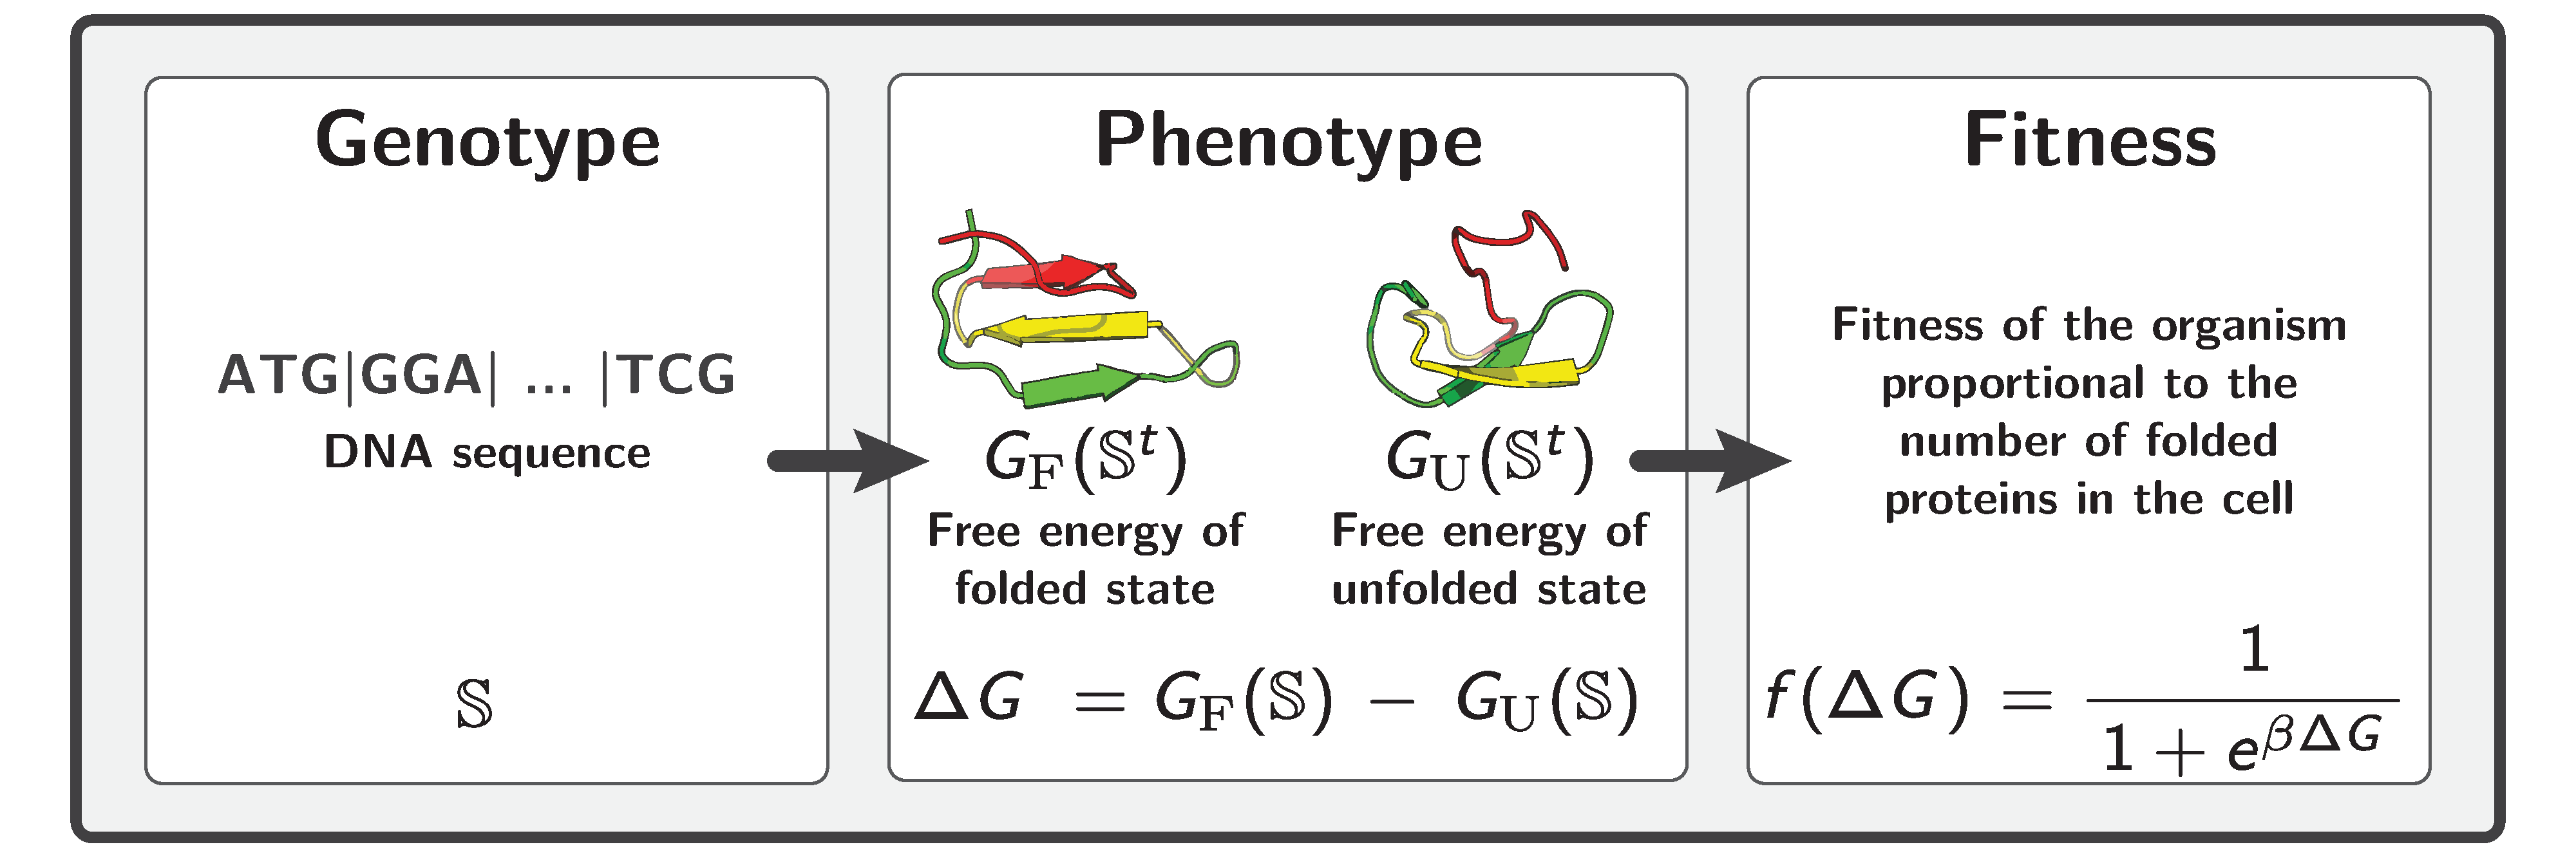
\includegraphics[width=165mm] {artworks/ModelSimuFold.pdf}
\end{center}
For each possible mutant ($t+1$ substitutions), we compute $\Delta G^{t+1}$ from the updated sequence $\mathbb{S}^{t+1}$, and subsequently the selection coefficient of the mutant:
\begin{equation}
s \left( \Delta G^{t}, \Delta G^{t+1} \right) = \dfrac{f(\Delta G^{t+1}) - f(\Delta G^{t})}{f(\Delta G^{t})}.
\end{equation}
The next change in the protein coding DNA and the time to next the event is chosen using Gillespie algorithm, according to the rates of substitution between codons:
\begin{equation}
{\submatrix_{\itoj}} = \mu_{\itoj} \dfrac{4 \Ne s \left( \Delta G^{t}, \Delta G^{t+1} \right)}{{1 - \e^{-4 \Ne s \left( \Delta G^{t}, \Delta G^{t+1} \right)} }}, 
\end{equation}
where ${\submatrix_{\itoj}} = \mu_{\itoj}$ in the case of synonymous substitutions.

\end{document}